\section{*untastic *esults que ahora es *didas *raining}

Los tutores famosos de un centro muy famoso donde la gente estudia programación de computadores (un ramo muy famoso) se están preparando para el verano, tonificando sus cuerpos con el objetivo de subir fotos de estilo \textit{fitness} a sus redes sociales. Para esto, están organizando sus rutinas de ejercicios en diccionarios, que se presentan a continuación:

\begin{itemize}
    \item El diccionario \texttt{rutinas} contiene como llave un tipo de rutina y su valor respectivo es una lista de tuplas, donde cada tupla tiene dos elementos: el nombre del ejercicio y su cantidad de repeticiones.
    
    \item El diccionario \texttt{usuarios} contiene como llave el nombre de un usuario y como valor una lista con los nombres de las rutinas que realizará en orden (como tipo string).
    
    \item El diccionario \texttt{series} contiene como llave el nombre de un tipo de rutina, y como valor la cantidad de rondas que tiene el entrenamiento. Por ejemplo, el entrenamiento \textit{Bravo} repite wdos veces los ejercicios asociados a él en el diccionario \texttt{rutinas}.
\end{itemize}

\begin{lstlisting}[style=consola]
# {tiporutina: [(ejercicio, repeticiones), ...]}
rutinas={'Alpha':[('Walking High Knees',20),
                  ('High Knees',20),
                  ('Kee Push-ups',20),
                  ('Walking Lunges',20)],
         'Bravo':[('Power Squats',30),
                  ('Knee Push-ups',20),
                  ('Leg Raises',10)],
         'Charlie':[('Jumping Jacks',20),
                    ('Knee Push-ups',10),
                    ('Power Squats',10),
                    ('4Count Burpees',10)]  }
\end{lstlisting}

\begin{lstlisting}[style=consola]
# {Nombre: [tiporutina, tiporutina, ...]}
usuarios={'Miguel':['Bravo','Charlie'],
          'Anghelo':['Alpha','Charlie'],
          'Diego':['Alpha','Alpha','Alpha']  }
\end{lstlisting}

\begin{lstlisting}[style=consola]
# {tiporutina: numeroderondas}
series={'Alpha':3,
        'Bravo':2,
        'Charlie':3}
\end{lstlisting}



\begin{enumerate}
    \item \texttt{quienes\_ejercitan(usuarios)}, donde \texttt{usuarios} es un diccionario con la estructura antes descrita. Esta función entrega un diccionario, donde la llave es el nombre de la rutina, y el valor es una lista, la cual contiene los nombres de las personas que realizan dicha rutina.

\begin{lstlisting}[style=consola]
>>> [*gente = quienes_ejercitan(usuarios)*]
>>> [*print(gente)*]
{'Bravo': ['Miguel'], 'Charlie': ['Miguel', 'Anghelo'],
'Alpha': ['Anghelo', 'Diego']}
\end{lstlisting}
\pagebreak[4]
    \item \texttt{rutina\_mas\_usada(usuarios)}, donde \texttt{usuarios} es un diccionario con la estructura antes descrita. Esta función entrega la rutina mas utilizada entre los usuarios.

\begin{lstlisting}[style=consola]
>>> [*la_mas_usada = rutina_mas_usada(usuarios)*]
>>> [*print(la_mas_usada)*]
'Alpha'
\end{lstlisting}

    \item \texttt{crear\_plantilla(rutinas, usuarios, series, nombre)} que reciba como parámetros los tres diccionarios \texttt{rutinas}, \texttt{usuarios} y \texttt{series} además de un string \texttt{nombre} con el nombre de un usuario. Esta función debe crear un archivo de texto llamado \texttt{rutina de X.txt} donde \texttt{X} es el nombre del usuario ingresado. \\Este archivo contiene agrupados los ejercicios y su cantidad de repeticiones (según el diccionario rutinas), que a la vez están agrupados en las rondas respectivas de cada entrenamiento (del diccionario series), donde además estas están agrupadas en el entrenamiento o rutina respectiva (de la lista que está asociada con el nombre del usuario en el diccionario \texttt{usuarios}). Este archivo de texto tiene al final un contador que indica cuantas repeticiones totales de ejercicios hizo el sujeto en cuestión. La función retorna None.
    \begin{figure}[H]
        \centering
        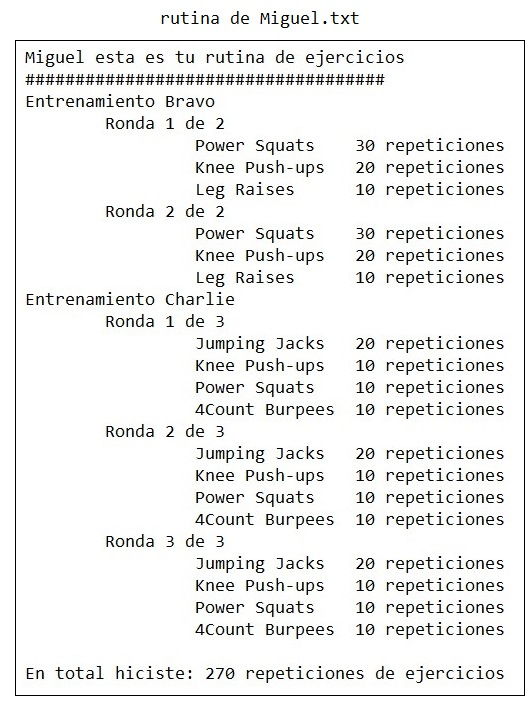
\includegraphics{Imagenes/planilla.jpg}
    \end{figure}

\end{enumerate}
